\begin{figure*}
  \centering
\begin{subfigure}[b]{\textwidth}
  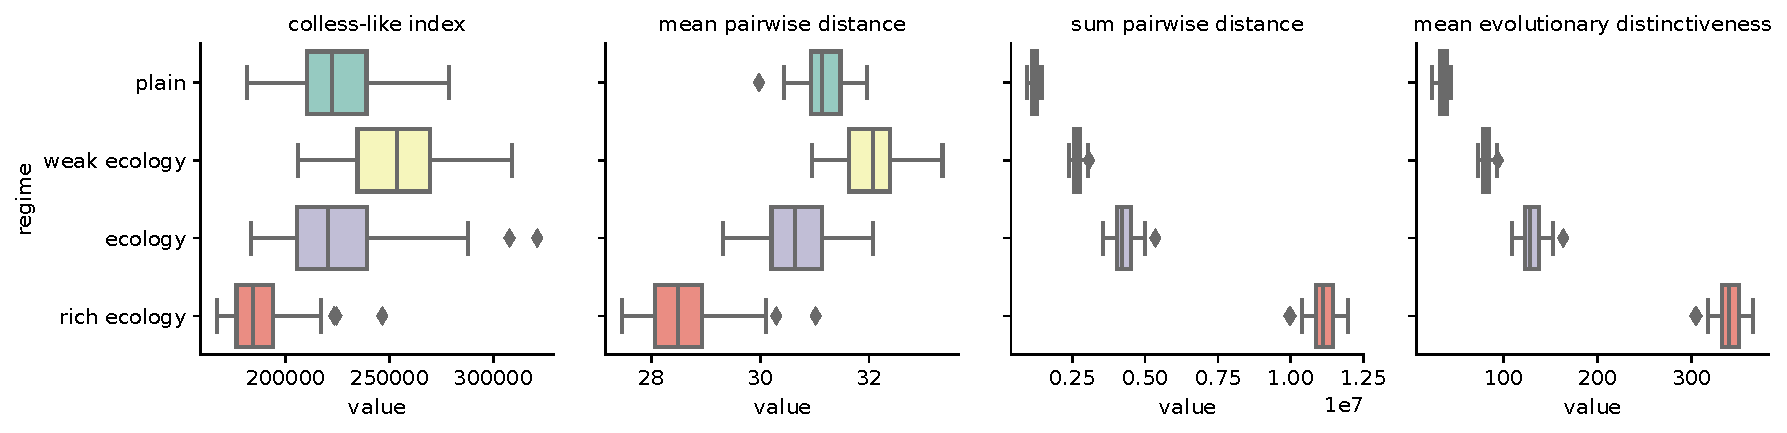
\includegraphics[width=\textwidth]{binder/binder/teeplots/col=phylometric+epoch=7+mut_distn=np.random.standard_normal+nuisance=spatial-structure+viz=boxplot+x=value+y=regime+ext=.pdf}
  \caption{ Distribution of phylometrics under the simple model.
    Sample sizes $n=50$.}
\end{subfigure}

\begin{subfigure}[b]{\textwidth}
  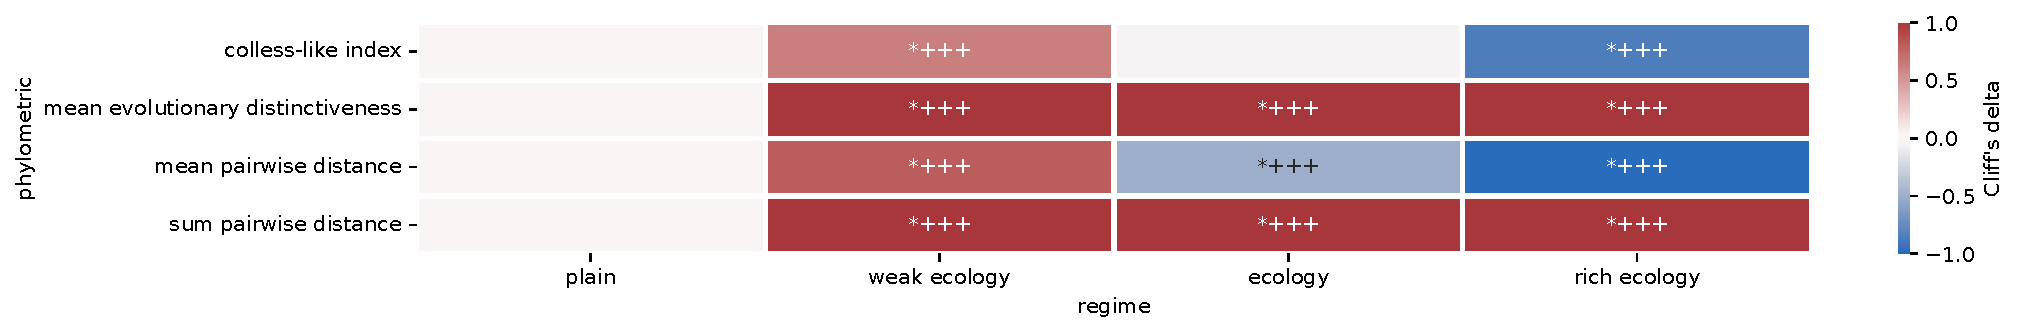
\includegraphics[width=\textwidth]{binder/binder/teeplots/epoch=7+mut_distn=np.random.standard_normal+spatial=true+viz=heatmap+x=regime+y=phylometric+ext=.pdf}
  \caption{Sizes of the effect of evolutionary regimes on each phylometric relative to ``plain'' baseline in the simple model.
    Sample sizes $n=50$.}
\end{subfigure}

\begin{subfigure}[b]{\textwidth}
  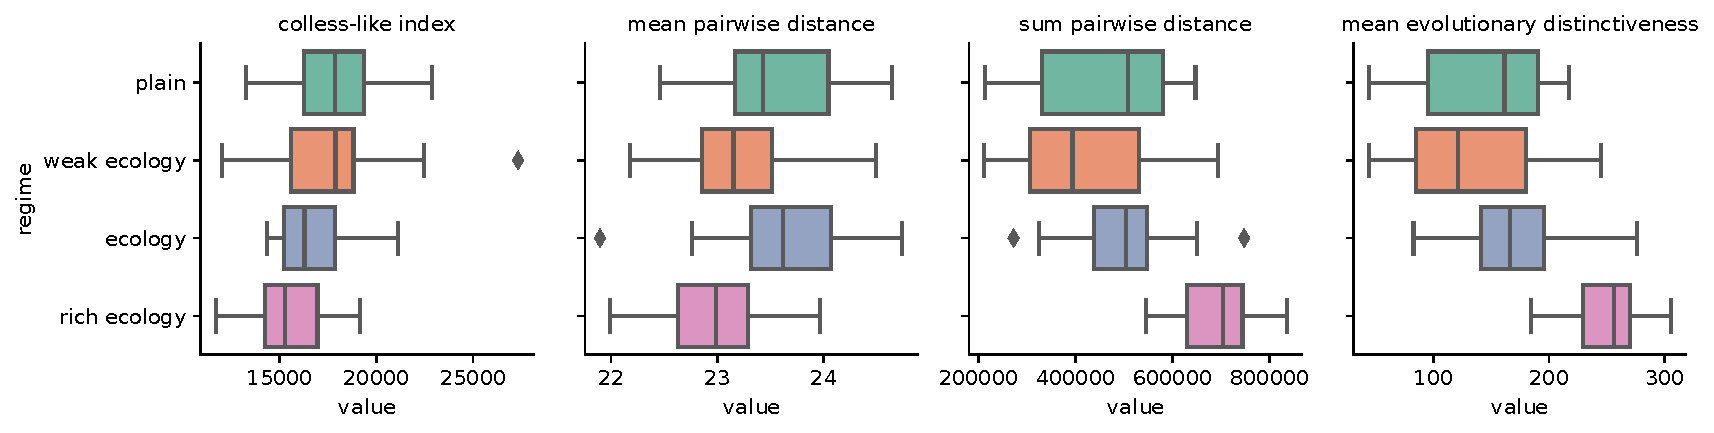
\includegraphics[width=\textwidth]{binder/binder/avida-individual/teeplots/col=phylometric+epoch=0+mut_distn=default+spatial=true+viz=boxplot+x=value+y=regime+ext=.pdf}
  \caption{ Distribution of phylometrics in Avida.
  Sample sizes $n=30$.}
\end{subfigure}%

\begin{subfigure}[b]{\textwidth}
  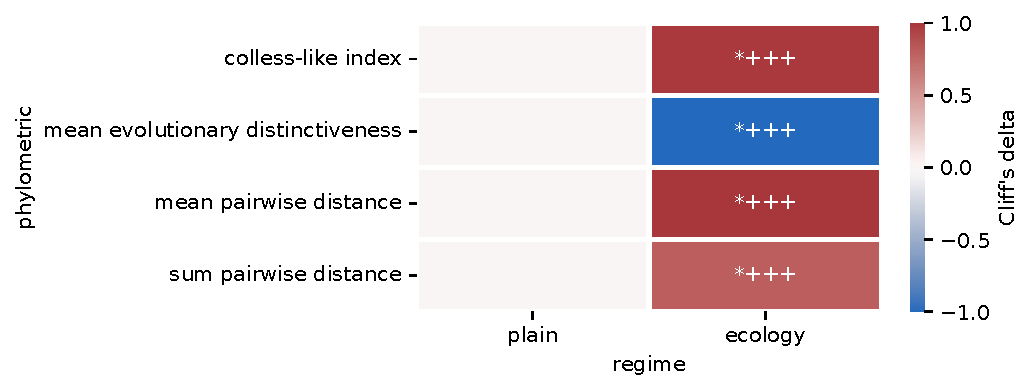
\includegraphics[width=\textwidth]{binder/binder/avida-individual/teeplots/epoch=0+mut_distn=default+spatial=true+viz=heatmap+x=regime+y=phylometric+ext=.pdf}
\caption{%
Sizes of the effect of evolutionary regimes on each phylometric relative to ``plain'' baseline in Avida.
    Sample sizes $n=30$.
}
\end{subfigure}
\vspace{1cm}


  \caption{%
    \textbf{Phylometric responses under spatial structure.}
    Distribution of phylometrics across the three surveyed ecological regimes and the control non-ecological regime---all with spatial population structure (i.e., island count 1,024 for simple model, toroidal population grid for Avida).
    Phylometrics were calculated on perfect-fidelity phylogenies.
    Note that nonparametric effect size normalization caps out to 1.0/-1.0 past the point of complete disbributional nonoverlap.
    For heatmap charts, +'s indicate small, medium, and large effect sizes using the Cliff's delta statistic and *'s indicate statistical significance at $\alpha = 0.05$ via Mann-Whitney U test.
    Results from simple model are for standard experimental conditions: gaussian mutation distribution at epoch 7 (generation 262,144).
    See Figure \ref{fig:perfect-tree-phylometrics-with-spatial-nuisance-sensitivity-analysis} for results under sensitivity analysis conditions.
  }
  \label{fig:perfect-tree-phylometrics-with-spatial-nuisance}
\end{figure*}
